\section{Auswertung}
\label{sec:Auswertung}

Die Werte der Bauteile in der untersuchten Schaltung betragen
\begin{align*}
  L &= \SI{10.11(003)}{\milli\henry}\,, \\
  C &= \SI{2.098(0006)}{\nano\farad}\,, \\
  R_1 &= \SI{48.1(01)}{\ohm}\,, \\
  R_2 &= \SI{509.5(05)}{\ohm}\,. \\
\end{align*}

Die mit dem Oszilloskop aufgenommene Spannung am Kondensator bei der gedämpften
Schwingung ist in Abbildung \ref{fig:einhuellende} zu sehen. Dort ist auch
bereits die Einhüllende eingezeichnet.

\begin{figure}
  \centering
  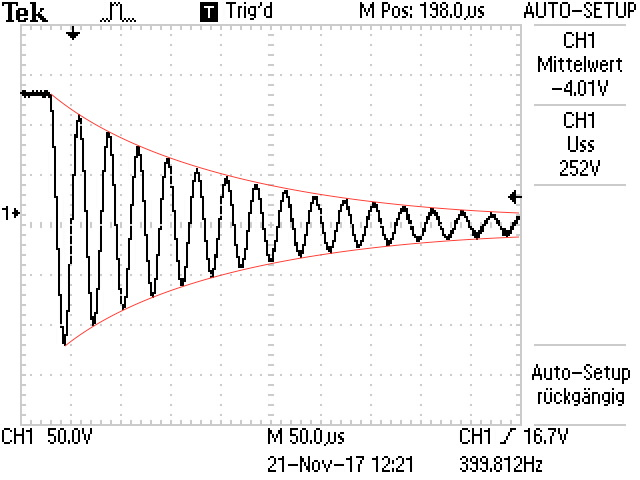
\includegraphics[width=300pt]{data/gedaempfte_schwingung2.JPG}
  \caption{Aufnahme des Spannungsverlaufs am Kondensator und Einhüllende bei der
  gedämpften Schwingung}
  \label{fig:einhuellende}
\end{figure}

Alle Spannungen am Oszilloskop wurden mit zehn
multipliziert dargestellt. Die aus der Kurve entnommenen Messwerte sind in Tabelle
\ref{tab:einhuellende} eingetragen.

\begin{table}
\centering
\caption{Messdaten zur gedämpften Schwingung des Schwingkreises}
\label{tab:einhuellende}
\begin{tabular}{c c c}
\toprule
$t/$µs & $10U_\mathrm{C}/$V & $U_\mathrm{C}/$V \\
\midrule
  1 & 132 & 13,2 \\
 29 & 112 & 11,2 \\
 58 &  94 &  9,4 \\
 88 &  80 &  8,0 \\
118 &  66 &  6,6 \\
147 &  58 &  5,8 \\
177 &  50 &  5,0 \\
206 &  42 &  4,2 \\
236 &  36 &  3,6 \\
265 &  30 &  3,0 \\
297 &  28 &  2,8 \\
324 &  24 &  2,4 \\
354 &  20 &  2,0 \\
382 &  18 &  1,8 \\
412 &  16 &  1,6 \\
441 &  14 &  1,4 \\
\bottomrule
\end{tabular}
\end{table}

Es wird eine nichtlineare Ausgleichsrechnung mit diesen Messwerten durchgeführt.
In diesem Fall gilt $U(t) \propto I(t)$ gemäß \eqref{eqn:ifunktion}, sodass die
Ausgleichsfunktion der Zuordnung
\begin{equation}
  U_\text{C}(t) = U_0 \exp(-2 \pi \mu t)
\end{equation}
folgt. Dabei gilt für µ der Zusammenhang
\begin{equation}
  \mu = \frac{R}{4 \pi L}\,.
  \label{eqn:mu}
\end{equation}
Der Widerstand R wird hier mit dem effektiven Dämpfungswiderstand $R_\text{eff}$ assoziiert, der
durch die Ausgleichsrechnung aus $\mu$ bestimmt werden kann.
In Abbildung \ref{fig:einhuellendefit} sind die abgelesenen Messwerte und der Graph
der konkreten Ausgleichsfunktion zu sehen.

\begin{figure}
  \centering
  \includegraphics{build/einhuellende.pdf}
  \caption{Auftragung von $U_\text{C}$/V gegen $t$/µs und Graph der Ausgleichsfunktion}
  \label{fig:einhuellendefit}
\end{figure}

Die Parameter ergeben sich hier zu
\begin{align*}
  U_0 &= \SI{13.04(011)}{\volt}\,, \\
  \mu &= \SI{861(012)}{\micro\second}\,,
\end{align*}
sodass für den effektiven Dämpfungswiderstand $R_\text{eff}$ nach \eqref{eqn:mu}
\begin{equation*}
  R_\text{eff} = \SI{109.4(0016)}{\ohm}
\end{equation*}
folgt. Die relative Unsicherheit beträgt 1.46\%. Die charakteristische
Abklingdauer $T_\text{ex}$ ist mit \eqref{eqn:abklingdauer} und \eqref{eqn:mu} dann
\begin{equation*}
  T_\text{ex} = \frac{2L}{R} = frac{1}{2\pi \mu} = \SI{184.8(0026)}{\micro\second}
\end{equation*}
mit einer relativen Unsicherheit von 1.41\%.

HIER NOCH INNENWIDERSTAND

Für den aperiodischen Grenzfall muss ein Widerstand $R_\text{ap}$ eingestellt werden.
Dieser wurde zu $\SI{3.550}{\kilo\ohm}$ bestimmt. Wird dieser Widerstand nach
\eqref{eqn:rap} bestimmt, so ergibt sich für ihn $\SI{4.390(0009)}{\kilo\ohm}$.
Dabei beträgt die absolute Unsicherheit $\SI{-840(9)}{\kilo\ohm}$.

Wie an \eqref{eqn:Ucfrequenz} ersichtlich ist, hängt die Kondensatorspannung von
der Frequenz ab. In Tabelle \ref{tab:amplitude} sind die aufgenommenen Messwerte
angegeben, um diese Abhängigkeit zu untersuchen. Es sei darauf hingewiesen, dass
ursprünglich Messwerte bereits ab ei

500	64.8		65
600	64.8		64
700	64.8		64
800	64.8		64
900	64.8		64
1000	66		63.5
1500	66		64.5
2000	66		64.5
3000	66.8		66
4000	66.8		64
5000	67.6		64
6000	67.6		64.5
7000	68.4		65
8000	69.2		65
9000	70.8		65
10000	72		63.5
15000	81		64.5
20000	98		64.5
21000	103		64.5
22000	108		64.5
23000	115		64.5
24000	121		64.5
25000	131		63.5
26000	140		63.5
27000	151		63.5
28000	165		63.5
29000	181		63.5
30000	197		63.5
31000	212		63.5
32000	230		63.5
33000	238		63.5
34000	234		63.5
35000	222		64
36000	202		64
37000	180		64
38000	160		64
39000	140		64
40000	128		64
41000	115		64
42000	103		64
43000	93		64
44000	85		64
45000	77		64
46000	72		64
47000	63.6		64
48000	59.2		64
49000	54.8		64
50000	51.6		64
60000	30		64
70000	19.4		64
80000	13.7		64
90000	10.4		64
100000	8.1		64
150000	2.91		64
200000	1.4		64
300000	0.29		64
